C++通过异常机制提供了通知和处理错误的框架。因为有些错误发生在设备上,或者在设备上启动工作时,所以异构编程还需要对错误级别进行管理。这些错误通常与主程序的执行不相关,因此不能与C++异常处理机制相集成。为了解决这个问题,需要有其他机制可以使异步错误像C++异常一样易于管理和控制。\par

图5-1展示了程序的两个组件:(1)主机代码运行顺序,以及执行和提交工作任务图(2)的异步置信国内和函数或对其他设备操作,与主程序的运行的依赖性。例子使用parallel\_for执行内核函数,并作为任务图的一部分异步执行,其他的操作会在第3、4和8章中再进行讨论。\par

\hspace*{\fill} \par %插入空行
图5-1 分离主程序和内核任务
\begin{center}
	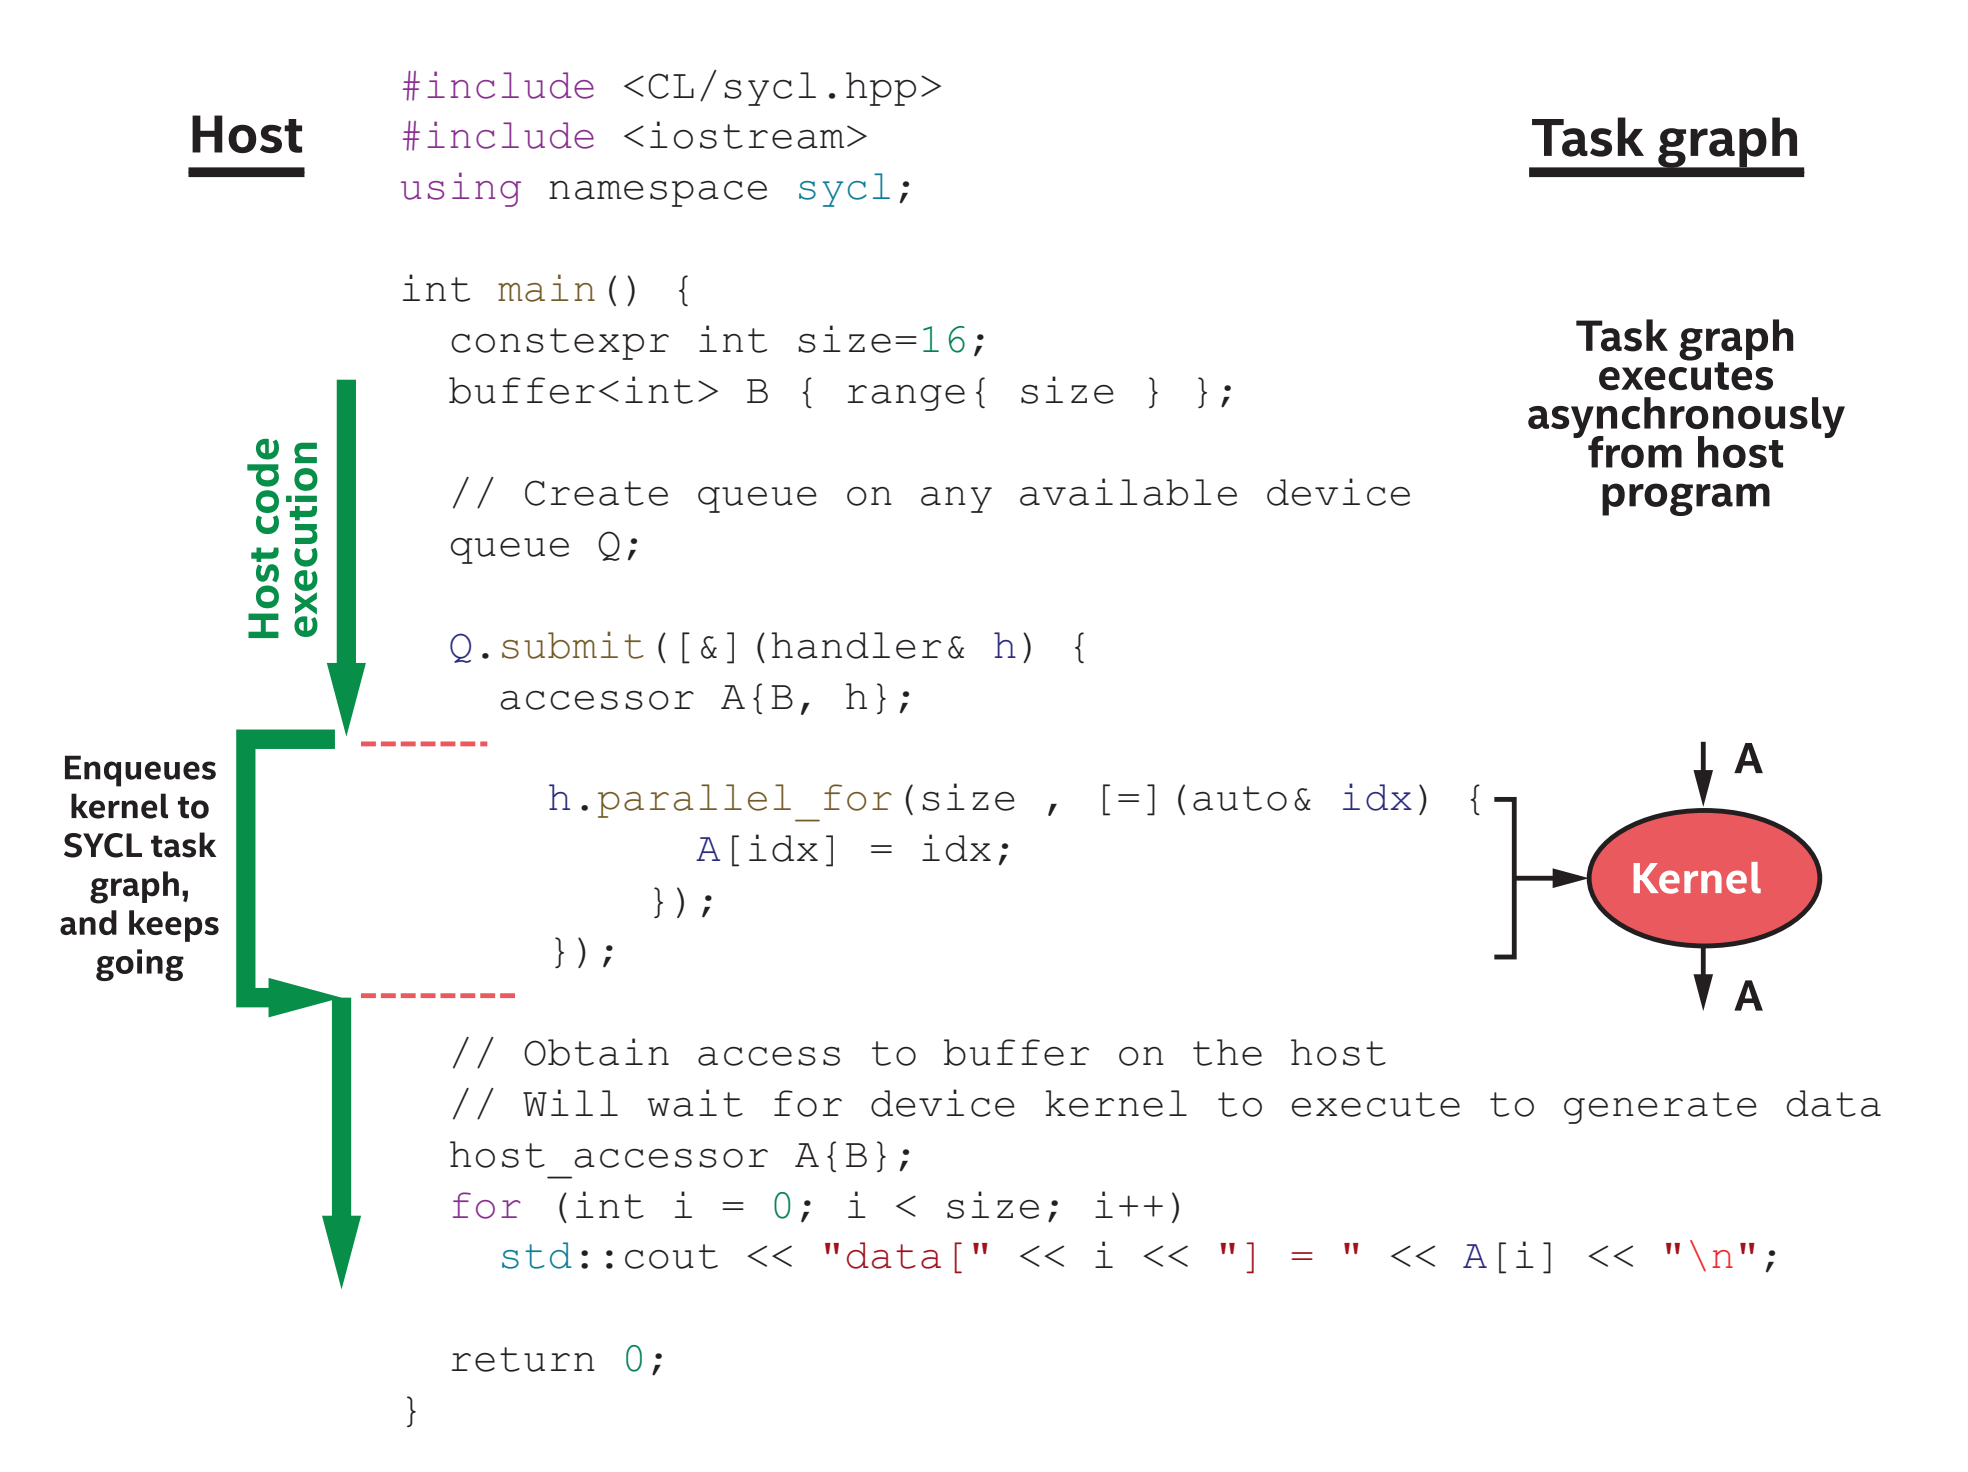
\includegraphics[width=1.0\textwidth]{content/chapter-5/images/2}
\end{center}

了解图5-1中左边和右边(主机和任务图)之间的区别,是理解同步和异步错误区别的关键。\par

主程序执行某个操作(如API调用或对象构造函数),在检测到错误条件时,就会发生同步错误。可以在图左侧的指令完成之前检测到,并且可以立即导将错误抛出。可以在图的左侧使用try-catch来包装指令,期望在try块结束(从而捕获)之前检测到try中操作的错误。C++异常机制就是为了处理这些错误而设计的。\par

当图5-1右侧出现异步错误,只有在执行任务中的操作才会检测到错误。当检测到异步错误时,主程序通常会继续执行,所以没有代码可以用try-catch来捕获这些错误。不放,有异步异常处理框架可以来处理这些错误。\par










